
%(BEGIN_QUESTION)
% Copyright 2006, Tony R. Kuphaldt, released under the Creative Commons Attribution License (v 1.0)
% This means you may do almost anything with this work of mine, so long as you give me proper credit

Beregn verdiene i kalibreringstabellen under for en fortrengertype nivåtransmitter som måler væskegrensesnitt (spesifikke vekter = 0.9 og 2.0), med kalibreringstoleranse $\pm$ 1\%:

$$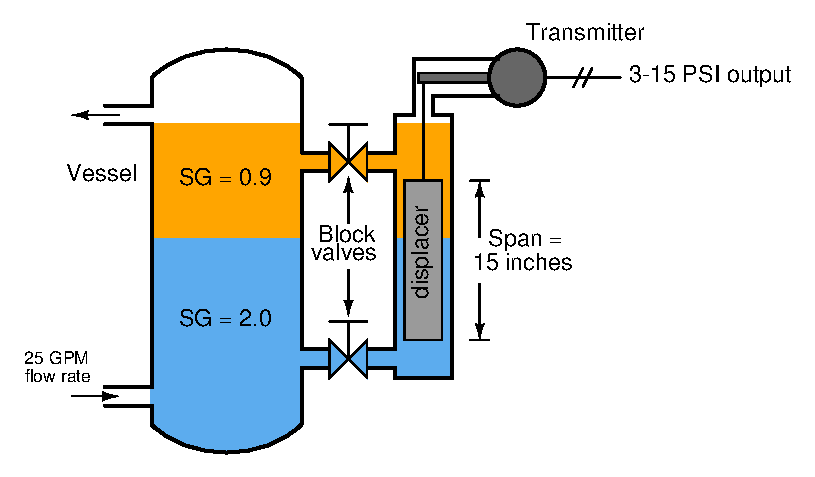
\includegraphics[width=15.5cm]{i00314x01.eps}$$

% No blank lines allowed between lines of an \halign structure!
% I use comments (%) instead, so that TeX doesn't choke.

$$\vbox{\offinterlineskip
\halign{\strut
\vrule \quad\hfil # \ \hfil & 
\vrule \quad\hfil # \ \hfil & 
\vrule \quad\hfil # \ \hfil & 
\vrule \quad\hfil # \ \hfil & 
\vrule \quad\hfil # \ \hfil & 
\vrule \quad\hfil # \ \hfil \vrule \cr
\noalign{\hrule}
%
% First row
Grensesnitt- & Prosent av & Oppdrifts- & Utgangssignal & Utgangssignal & Utgangssignal \cr
%
% Another row
nivå (in) & spenn (\%) & kraft (lbs) & ideelt (PSI) & min. (PSI) & maks. (PSI) \cr
%
\noalign{\hrule}
%
% Another row
  & 0 &  &  &  &  \cr
%
\noalign{\hrule}
%
% Another row
  & 10 &  &  &  &  \cr
%
\noalign{\hrule}
%
% Another row
  & 25 &  &  &  &  \cr
%
\noalign{\hrule}
%
% Another row
  & 50 &  &  &  &  \cr
%
\noalign{\hrule}
%
% Another row
  & 75 &  &  &  &  \cr
%
\noalign{\hrule}
%
% Another row
  & 90 &  &  &  &  \cr
%
\noalign{\hrule}
%
% Another row
  & 100 &  &  &  &  \cr
%
\noalign{\hrule}
} % End of \halign 
}$$ % End of \vbox

Anta følgende fortrengerdata:

\begin{itemize}
\item{} Form: {\it sylindrisk}
\item{} Lengde = 15 tommer
\item{} Diameter = 2 tommer
\item{} Tørrvekt = 4.5 lbs
\end{itemize}

\vskip 10pt

Vis all matematisk utregning slik at instruktøren kan kontrollere den konseptuelle gyldigheten av metoden(e) dine.  En god kontroll er å verifisere at alle mellomregninger har fysisk mening.  {\bf Hvis du virkelig forstår hva du gjør, vil du kunne identifisere riktig måleenhet for hvert mellomresultat og vise hvor tallet gjelder i scenariet}.

\vskip 20pt \vbox{\hrule \hbox{\strut \vrule{} {\bf Forslag til sokratisk diskusjon} \vrule} \hrule}

\begin{itemize}
\item{} To teknikere diskuterer virkemåten til en fortrengertype nivåtransmitter.  Den ene mener statisk trykk i prosesskaret påvirker nøyaktigheten, den andre mener det ikke gjør det.  Hvem har rett, og hvorfor?
\item{} Demonstrer hvordan man kan {\it estimere} numeriske svar uten kalkulator.
\end{itemize}

\underbar{file i00314}
%(END_QUESTION)





%(BEGIN_ANSWER)

\noindent
{\bf Delvis svar:}

% No blank lines allowed between lines of an \halign structure!
% I use comments (%) instead, so that TeX doesn't choke.

$$\vbox{\offinterlineskip
\halign{\strut
\vrule \quad\hfil # \ \hfil & 
\vrule \quad\hfil # \ \hfil & 
\vrule \quad\hfil # \ \hfil & 
\vrule \quad\hfil # \ \hfil & 
\vrule \quad\hfil # \ \hfil & 
\vrule \quad\hfil # \ \hfil \vrule \cr
\noalign{\hrule}
%
% First row
Grensesnitt- & Prosent av & Oppdrifts- & Utgangssignal & Utgangssignal & Utgangssignal \cr
%
% Another row
nivå (in) & spenn (\%) & kraft (lbs) & ideelt (PSI) & min. (PSI) & maks. (PSI) \cr
%
\noalign{\hrule}
%
% Another row
0 & 0 &  &  &  & 3.12 \cr
%
\noalign{\hrule}
%
% Another row
 & 10 &  &  & 4.08 &  \cr
%
\noalign{\hrule}
%
% Another row
 & 25 &  &  &  &  \cr
%
\noalign{\hrule}
%
% Another row
 & 50 & 2.469 &  &  &  \cr
%
\noalign{\hrule}
%
% Another row
11.25 & 75 &  &  &  &  \cr
%
\noalign{\hrule}
%
% Another row
 & 90 &  &  &  &  \cr
%
\noalign{\hrule}
%
% Another row
 & 100 &  & 15 &  &  \cr
%
\noalign{\hrule}
} % End of \halign 
}$$ % End of \vbox

%(END_ANSWER)





%(BEGIN_NOTES)

Her er to ``tankeeksperiment''-tilfeller vist for å finne LRV- og URV-verdier:

$$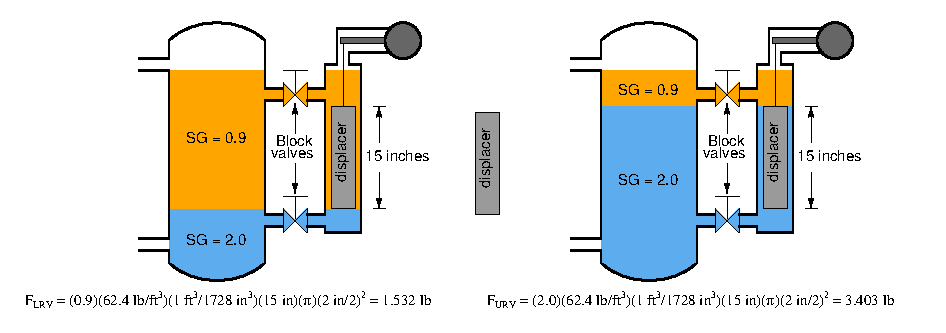
\includegraphics[width=15.5cm]{i00314x02.eps}$$

% No blank lines allowed between lines of an \halign structure!
% I use comments (%) instead, so that TeX doesn't choke.

$$\vbox{\offinterlineskip
\halign{\strut
\vrule \quad\hfil # \ \hfil & 
\vrule \quad\hfil # \ \hfil & 
\vrule \quad\hfil # \ \hfil & 
\vrule \quad\hfil # \ \hfil & 
\vrule \quad\hfil # \ \hfil & 
\vrule \quad\hfil # \ \hfil \vrule \cr
\noalign{\hrule}
%
% First row
Grensesnitt- & Prosent av & Oppdrifts- & Utgangssignal & Utgangssignal & Utgangssignal \cr
%
% Another row
nivå (in) & spenn (\%) & kraft (lbs) & ideelt (PSI) & min. (PSI) & maks. (PSI) \cr
%
\noalign{\hrule}
%
% Another row
0 & 0 & 1.532 & 3 & 2.88 & 3.12 \cr
%
\noalign{\hrule}
%
% Another row
1.5 & 10 & 1.719 & 4.2 & 4.08 & 4.32 \cr
%
\noalign{\hrule}
%
% Another row
3.75 & 25 & 2.000 & 6 & 5.88 & 6.12 \cr
%
\noalign{\hrule}
%
% Another row
7.5 & 50 & 2.469 & 9 & 8.88 & 9.12 \cr
%
\noalign{\hrule}
%
% Another row
11.25 & 75 & 2.937 & 12 & 11.88 & 12.12 \cr
%
\noalign{\hrule}
%
% Another row
13.5 & 90 & 3.218 & 13.8 & 13.68 & 13.92 \cr
%
\noalign{\hrule}
%
% Another row
15 & 100 & 3.405 & 15 & 14.88 & 15.12 \cr
%
\noalign{\hrule}
} % End of \halign 
}$$ % End of \vbox

\vskip 10pt

Flowraten på 25 GPM er overflødig informasjon, inkludert for å utfordre studentene til å avgjøre om informasjonen er relevant for oppgaven.

%INDEX% Measurement, interface level: displacer (buoyancy)

%(END_NOTES)
